\documentclass[11pt,a4paper]{article}
\usepackage[T1]{fontenc}
\usepackage[margin=2.3cm]{geometry}
\usepackage{amsmath,amssymb}
\usepackage{graphicx}
\usepackage[dvipsnames]{xcolor}
\usepackage{enumitem}
\usepackage[colorlinks=true,linkcolor=blue,urlcolor=blue]{hyperref}
\setlength{\parskip}{0.6em}
\setlength{\parindent}{0pt}
\begin{document}

\begin{center}{\LARGE\bfseries openpressurecooker}\\[0.4em]{\large Why a pressure cooker cooks faster, from boiling point to a simulation you can check.}\\[0.2em]\small PAN IIT OSS explainer \textbullet{} middle school to higher secondary (levels 2-4)\end{center}

\section*{Why this exists}
A pressure cooker is a small, sealed steam engine's cousin: it traps steam, the pressure rises, and water boils hotter. This explainer shows the physics, from one relation between pressure and boiling point to a simulation you can check, so you can build it yourself.

\section*{The end goal}
Show why a pressure cooker cooks faster using pressure and boiling point. The end goal is to show why a pressure cooker cooks faster using pressure and boiling point: a hotter pot makes cooking chemistry go several times faster. Education only: never modify or block the valves of real equipment.

\section*{How the three sessions build up}
\begin{enumerate}[nosep]
\item \textbf{Session 1: Pressure changes the boiling point} (Level 1, conceptual interactive model, 60 min).
\item \textbf{Session 2: The boiling-point curve from physics} (Level 2, mathematical engineering model, 75 min).
\item \textbf{Session 3: Simulating heating, venting and cooking} (Level 3, simulation and validation, 90 min).
\end{enumerate}

\section{Session 1: Pressure changes the boiling point}

\subsection*{A. Real-world problem}
Lentils take about 40 minutes in an open pot and a much shorter time in a pressure cooker, on the same flame. The cooker does not make the flame hotter. What does the sealed lid change? This is a simplified teaching model for understanding, not a guide for using or altering real equipment: never modify, block or remove the valves of a real cooker.

\subsection*{B. Concept and theory}
Water boils when bubbles of steam can form against the pressure around the water. At the pressure of the air at sea level, 101.3 kPa, that happens at 100 degrees C. If the pressure is higher, bubbles need a hotter liquid, so the boiling point rises. In an open pot the steam escapes, so the pressure stays at one atmosphere and the water cannot get hotter than 100 degrees C however big the flame (extra heat only makes more steam). A cooker has a sealed lid and a weighted valve: steam collects, the pressure rises until the valve lifts, and then it holds a set pressure. A gauge reads the pressure above the air, so absolute pressure = gauge + 101.325 kPa. We read boiling points from a small table of approximate steam-table values. Chemistry (softening, breaking down) goes faster when it is hotter; a rule of thumb says the rate roughly doubles for each 10 degrees C, so speed factor = 2 to the power (T - 100) / 10. It is a rule of thumb, not an exact law.

\begin{itemize}[nosep]
\item P\_gauge: pressure above the air, as shown by a gauge (kPa)
\item P\_abs: absolute pressure = gauge + 101.325 (kPa)
\item T: boiling point at that pressure (degrees C)
\item f: cooking speed factor compared with 100 degrees C (no unit)
\item t\_open, t\_cooker: cooking time in an open pot and in the cooker (min)
\end{itemize}

\begin{equation*}
P_{\mathrm{abs}}=P_{\mathrm{gauge}}+101.325\ \mathrm{kPa}
\end{equation*}

\begin{equation*}
f=2^{(T-100)/10}
\end{equation*}

\begin{equation*}
t_{\mathrm{cooker}}=\frac{t_{\mathrm{open}}}{f}
\end{equation*}

\begin{center}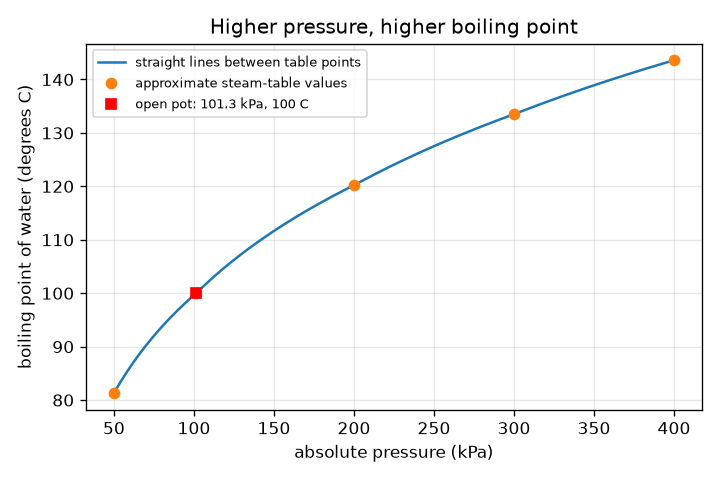
\includegraphics[width=0.85\linewidth]{figures/s01_boiling_vs_pressure.png}\\\small Boiling point against absolute pressure: higher pressure, higher boiling point, with a flattening curve.\end{center}

\subsection*{E. Worked example}
A cooker holds 100 kPa gauge. What is the absolute pressure, the boiling point, the speed factor, and the time for a recipe that needs 40 minutes in an open pot?
\begin{enumerate}[nosep]
\item Absolute pressure = 100 + 101.325 = 201.3 kPa.
\item The table has 200 kPa at 120.2 degrees C and 300 kPa at 133.5 degrees C, so 201.3 kPa is just above 200: boiling point about 120.4 degrees C.
\item Speed factor = 2\textasciicircum{}((120.4 - 100) / 10) = 2\textasciicircum{}2.04 = 4.12.
\item Time = 40 / 4.12 = 9.7 minutes.
\end{enumerate}
\textbf{Answer.} Absolute pressure 201.3 kPa, boiling point about 120.4 degrees C, about 4.1 times faster, so about 9.7 minutes.

\subsection*{F. Questions}
\begin{enumerate}[nosep]
\item \textbf{Conceptual.} Why can an open pot never get the water hotter than about 100 degrees C, even on a huge flame? What does the extra heat do instead?
\item \textbf{Numerical.} A cooker holds 150 kPa gauge. Find the absolute pressure, the boiling point from the table, the speed factor and the time for a recipe that needs 60 minutes in an open pot.
\item \textbf{Graph and simulation interpretation.} On the boiling-point graph, how much does the boiling point rise between 101 and 200 kPa, and between 200 and 300 kPa? What does the change in steepness tell you about adding more pressure?
\item \textbf{Design and optimisation challenge.} Design: choose a gauge pressure (in whole 5 kPa steps) so that a 40 minute open-pot recipe takes 12 minutes or less, and say what limits you from simply choosing a much higher pressure.
\end{enumerate}

\section{Session 2: The boiling-point curve from physics}

\subsection*{A. Real-world problem}
Session 1 read boiling points from a table. Where do the table numbers come from, and how heavy must the weight on a cooker's valve be to hold the pressure at 100 kPa above the air? We derive the boiling-point curve from one physical relation and then size the weight. This is a simplified educational calculation, not a design method: never modify, block or remove the valves of real equipment.

\subsection*{B. Concept and theory}
At the boiling point, liquid and vapour are in equilibrium, and the pressure and temperature are linked. Treating the vapour as an ideal gas, ignoring the small volume of the liquid, and taking the molar latent heat L of vaporisation as constant gives the Clausius-Clapeyron relation: ln(P2/P1) = (L/R)(1/T1 - 1/T2), with temperatures in kelvin. For water, L is about 40.7 kJ/mol near 100 degrees C, R = 8.314 J/(mol K), and the reference point is P1 = 101.325 kPa at T1 = 373.15 K. Solving for T2 gives the boiling point at a pressure P2, and solving for P2 gives the vapour pressure at a temperature. The relation is approximate: L changes a little with temperature and steam is not perfectly ideal, so we compare with a few approximate steam-table values (about 100 degrees C at 101.3 kPa, about 120 degrees C at about 200 kPa absolute). Gauge pressure = absolute - 101.325 kPa; physics uses absolute. For cooking, the rule of thumb is that the rate roughly doubles for each 10 degrees C rise (a Q10 of 2). A weighted valve lifts when the pressure force on its opening equals the weight: P\_gauge x A = m g, with A = pi d\textasciicircum{}2 / 4.

\begin{itemize}[nosep]
\item P1, P2: absolute pressures (kPa)
\item T1, T2: boiling temperatures at P1 and P2 (K)
\item L: molar latent heat of vaporisation of water, about 40.7 (kJ/mol (40700 J/mol))
\item R: gas constant 8.314 (J/(mol K))
\item Q10: factor by which a rate grows for +10 degrees C, taken as 2 (no unit)
\item m, d, A: valve mass, opening diameter and its area (kg, m, m\textasciicircum{}2)
\item g: gravitational acceleration 9.81 (m/s\textasciicircum{}2)
\end{itemize}

\begin{equation*}
\ln\frac{P_2}{P_1}=\frac{L}{R}\left(\frac{1}{T_1}-\frac{1}{T_2}\right)
\end{equation*}

\begin{equation*}
T_2=\left(\frac{1}{T_1}-\frac{R}{L}\ln\frac{P_2}{P_1}\right)^{-1}
\end{equation*}

\begin{equation*}
P_{\mathrm{abs}}=P_{\mathrm{gauge}}+101.325\ \mathrm{kPa},\qquad f=Q_{10}^{(T-100)/10}
\end{equation*}

\begin{equation*}
P_{\mathrm{gauge}}A=mg,\qquad A=\frac{\pi d^2}{4}\ \Rightarrow\ m=\frac{P_{\mathrm{gauge}}A}{g}
\end{equation*}

\begin{center}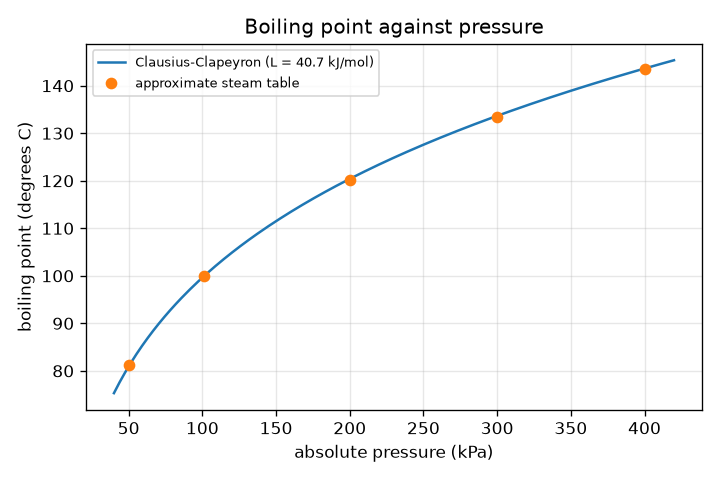
\includegraphics[width=0.85\linewidth]{figures/s02_clausius_clapeyron.png}\\\small Clausius-Clapeyron boiling-point curve with approximate steam-table points.\end{center}

\subsection*{E. Worked example}
Find the boiling point at 100 kPa gauge from Clausius-Clapeyron, the cooking rate factor, and the valve mass needed for a 4 mm opening.
\begin{enumerate}[nosep]
\item Absolute pressure P2 = 100 + 101.325 = 201.325 kPa, so P2 / P1 = 1.9868 and ln = 0.6865.
\item (R / L) ln = 8.314 / 40700 x 0.6865 = 1.4024e-4 per K. 1/T1 = 1/373.15 = 2.6799e-3 per K.
\item 1/T2 = 2.6799e-3 - 1.4024e-4 = 2.5397e-3, so T2 = 393.76 K = 120.6 degrees C. (The approximate steam-table value near 200 kPa is 120.2 degrees C.)
\item Rate factor = 2\textasciicircum{}((120.6 - 100) / 10) = 4.17, so a 40 minute recipe is about 9.6 minutes.
\item Valve: A = pi (0.004)\textasciicircum{}2 / 4 = 1.2566e-5 m\textasciicircum{}2. m = 100000 x 1.2566e-5 / 9.81 = 0.1281 kg = 128 g.
\end{enumerate}
\textbf{Answer.} Boiling point about 120.6 degrees C (steam table about 120.2), rate factor 4.17, and a 4 mm opening needs about 128 g of valve weight.

\subsection*{F. Questions}
\begin{enumerate}[nosep]
\item \textbf{Conceptual.} Why must the Clausius-Clapeyron relation use absolute temperature in kelvin and absolute pressure, not the gauge reading?
\item \textbf{Numerical.} Use Clausius-Clapeyron to find the boiling point at 50 kPa absolute (for example high on a mountain). Compare with the approximate table value 81.3 degrees C.
\item \textbf{Graph and simulation interpretation.} From the first figure, in which range of pressure does the Clausius-Clapeyron curve and the steam-table points agree best, and where do they differ most? Suggest why.
\item \textbf{Design and optimisation challenge.} Design: a cooker has a 5 mm valve opening. Choose a valve mass that holds 100 kPa gauge, say how the gauge pressure changes if the mass is 10 percent too heavy, and give the new boiling point.
\end{enumerate}

\section{Session 3: Simulating heating, venting and cooking}

\subsection*{A. Real-world problem}
How long does a cooker take to heat up, how much water does it lose, and how much faster does it really cook lentils than an open pot? We build a model with three parts and then try to break it: validate it against things we can calculate by hand, ask how sensitive it is, and see what a blocked vent would do in the model. This is a simplified educational model, not a design tool, and no instructions follow from it: never modify, block or remove the valves of real equipment.

\subsection*{B. Concept and theory}
Lumped model: one uniform water temperature T. The pot holds water of mass m and has heat capacity C = m cp + C\_pot. Heating: net power eta P (heater power P and efficiency eta). The headspace of volume V is full of saturated steam, an ideal gas: its mass is m\_s = psat(T) V M / (R T), with psat from Clausius-Clapeyron. The water-pot-steam enthalpy is H(T) = C T + L\_mass m\_s(T), so heating follows dH/dt = eta P until T reaches the regulator boiling point T\_b = Tsat(P\_atm + gauge). Then the regulator vents: the user turns the heat down to a hold power eta h P (h = 0.25), all of it makes steam that leaves, so the pressure and T stay fixed and water is lost at eta h P / L\_mass kg per second. Cooking: an Arrhenius rate k(T) = exp(-Ea/R (1/T - 1/T\_ref)) equals 1 at 100 degrees C; doneness D is the integral of k over time in equivalent boil minutes, and lentils are done at D = 40. We choose Ea = 82.4 kJ/mol, which gives a rate that about doubles for 10 degrees C near 100 degrees C (an illustrative value, not a measured one). The open pot is the same model with pressure 101.325 kPa and no sealed headspace. Failure case: if the vent is blocked, the heater keeps adding energy, T keeps rising and the pressure follows psat(T), rising at dP/dt = (psat L / (R T\textasciicircum{}2)) dT/dt. Real cookers have independent safety valves for exactly this reason.

\begin{itemize}[nosep]
\item T: uniform water temperature (K)
\item C: heat capacity of water plus pot, 4886 (J/K)
\item eta, P, h: heater efficiency (0.8), heater power (1000), hold fraction (0.25) (-, W, -)
\item V, m\_s: headspace volume (3 L) and its steam mass (m\textasciicircum{}3, kg)
\item L\_mass: latent heat per kg, L / M = 2.26e6 (J/kg)
\item Ea, k, D: activation energy, relative rate, doneness (J/mol, -, equivalent minutes)
\item gauge, T\_b: regulator setting and boiling point at that pressure (kPa, K)
\end{itemize}

\begin{equation*}
H(T)=C\,T+L_{\mathrm{mass}}\,m_s(T),\qquad m_s=\frac{p_{\mathrm{sat}}(T)\,V\,M}{R\,T}
\end{equation*}

\begin{equation*}
\frac{dH}{dt}=\eta P\ \ (T<T_b),\qquad \dot m_{\mathrm{vent}}=\frac{\eta h P}{L_{\mathrm{mass}}}\ \ (T=T_b)
\end{equation*}

\begin{equation*}
k(T)=\exp\!\left[-\frac{E_a}{R}\left(\frac{1}{T}-\frac{1}{373.15}\right)\right],\qquad D=\int k\,\frac{dt}{60}
\end{equation*}

\begin{equation*}
t_{\mathrm{heat}}\approx\frac{C\,(T_b-T_0)}{\eta P},\qquad \frac{dP}{dt}=\frac{p_{\mathrm{sat}}L}{R\,T^2}\,\frac{dT}{dt}
\end{equation*}

\begin{center}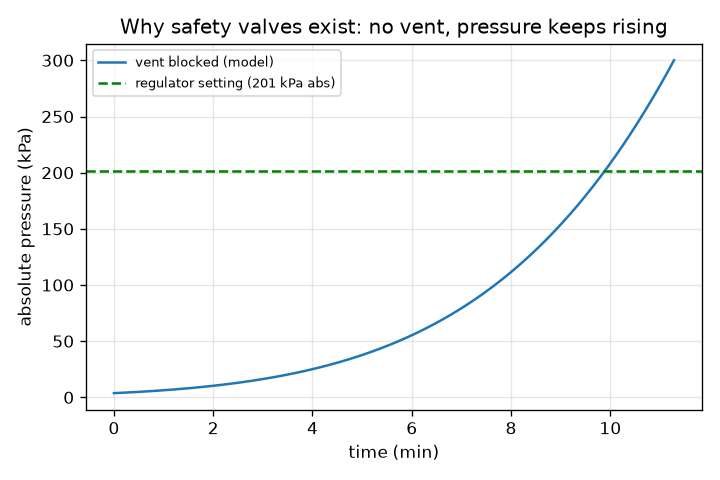
\includegraphics[width=0.85\linewidth]{figures/s03_blocked_vent.png}\\\small Failure case in the model: with no vent, pressure rises without limit.\end{center}

\subsection*{E. Worked example}
For 1 kg of water, a 1000 W heater at 80 percent efficiency, a pot heat capacity of 700 J/K, a 3 L headspace and a 100 kPa gauge regulator, find the hand heating time from 25 degrees C to boiling, the steam in the headspace, and compare with the simulation.
\begin{enumerate}[nosep]
\item C = 1 x 4186 + 700 = 4886 J/K. T\_b = 393.76 K = 120.61 degrees C, so the rise is 95.61 K.
\item Hand heating time = 4886 x 95.61 / (0.8 x 1000) = 584 s = 9.73 minutes.
\item Steam in the headspace at 120.6 degrees C: m\_s = 201325 x 0.003 x 0.018015 / (8.314 x 393.76) = 3.32 g.
\item Latent energy to make it: 3.32e-3 x 2.26e6 = 7.5 kJ, which takes 7.5e3 / 800 = about 9 s more.
\item The simulation gives boiling at 9.90 minutes (594 s): 584 s + about 10 s, within 2 percent of the hand formula, and the energy balance closes to better than 1e-6.
\end{enumerate}
\textbf{Answer.} Hand estimate 9.73 minutes, simulation 9.90 minutes (the headspace steam costs about 10 s); 3.32 g of steam; the cooker then finishes the lentils at 18.3 minutes against 46.3 minutes for the open pot.

\subsection*{F. Questions}
\begin{enumerate}[nosep]
\item \textbf{Conceptual.} Why does the cooker plateau at about 120.6 degrees C instead of continuing to heat up, and what happens to the extra energy once it reaches the plateau?
\item \textbf{Numerical.} For 2 kg of water, a 1500 W heater at 80 percent efficiency, 700 J/K pot and a regulator at 100 kPa gauge, estimate the heating time with the hand formula, ignoring the headspace.
\item \textbf{Graph and simulation interpretation.} On the doneness graph, estimate the slope of each pot's line after boiling starts, and use it to explain why the cooker finishes far sooner even though it boils later.
\item \textbf{Design and optimisation challenge.} Design: choose a regulator setting and heater power so that the lentils are done in at most 20 minutes and the water loss stays below 60 g. Use the sensitivity tables from the lesson and state the trade-off.
\end{enumerate}

\section{Real-world mini-project}
\textbf{Choose the whistle time for lentils.} A recipe says lentils need 40 minutes of simmering in an open pot after it starts boiling. Your cooker's regulator can be set to different gauge pressures. Use \texttt{cooker\_hold\_minutes(40, gauge)} from Session 3 to find how many minutes the cooker must hold pressure (counted from when the regulator starts venting) for gauge settings of 50, 75, 100 and 150 kPa. Compare with the shortcut 40 divided by the Q10 speed factor, and say why the simulation gives a shorter time. This is a model for learning: real timings depend on the food, the quantity and the equipment, so follow the maker's instructions and never change a valve.

\section{The path ahead}
\begin{enumerate}[nosep]
\item \textbf{Session 4: Real steam properties.} A saturation-pressure function with a temperature-dependent latent heat or a fitted equation, compared with tabulated data.
\item \textbf{Session 5: Heat loss and natural release.} A simulation extended with a heat-loss term and a cool-down phase after the heat is off.
\item \textbf{Session 6: Food with an inside.} A radial diffusion solver coupled to the cooking rate.
\item \textbf{Session 7: Altitude and the open pot.} The open-pot model with atmospheric pressure as an input, and a cooker setting that restores the sea-level time.
\item \textbf{Session 8: Relief devices in the model.} A second relief valve set above the regulator that opens in the blocked case, with the pressure traced over time.
\end{enumerate}

\section{Answers and hints}

\subsection*{Session 1}
\begin{enumerate}[nosep]
\item \textbf{Conceptual.} Hint: Think about where the steam goes and what the pressure around the water is. Solution: In an open pot the pressure stays at one atmosphere because the steam escapes. At that pressure the water boils at 100 degrees C, and any extra heat goes into turning more water into steam (latent heat), not into raising the temperature. To get hotter water the pressure has to be raised, which is what the sealed cooker does.
\item \textbf{Numerical.} Hint: Add 101.325 first, then interpolate between 200 and 300 kPa. Solution: Absolute = 251.3 kPa. The boiling point is between 120.2 (200 kPa) and 133.5 degrees C (300 kPa): about 127.7 degrees C. Speed factor = 2\textasciicircum{}(27.7/10) = 6.8. Time = 60 / 6.8 = about 8.8 minutes. Sanity check: for the same 40 minute recipe, 150 kPa gives 5.9 minutes against 9.7 at 100 kPa, so more pressure means a hotter pot and a shorter time, as expected.
\item \textbf{Graph and simulation interpretation.} Hint: Read the table points: 100, 120.2 and 133.5 degrees C. Solution: From 101.3 to 200 kPa it rises about 20 degrees C (100 to 120.2), roughly 0.20 degrees C per kPa. From 200 to 300 kPa it rises 13.3 degrees C, about 0.13 degrees C per kPa. The curve flattens, so each extra kPa buys less temperature: a much higher pressure (and a stronger, more dangerous vessel) gives diminishing returns.
\item \textbf{Design and optimisation challenge.} Hint: You need a speed factor of at least 40 / 12 = 3.33; find the temperature for that, then the pressure. Solution: A factor of 3.33 needs a boiling point of at least 100 + 10 log2(3.33) = 117.4 degrees C. The table gives that at about 82 kPa gauge (11.8 min at 82 kPa, 12.07 at 80 kPa), so choose 85 kPa (about 11.4 minutes). Limits: a higher pressure needs a stronger vessel and a heavier valve, spends more energy, can overcook or break up the food, and the benefit flattens with pressure. Real cookers have fixed, tested settings; this is a teaching calculation, never a reason to change a valve.
\end{enumerate}

\subsection*{Session 2}
\begin{enumerate}[nosep]
\item \textbf{Conceptual.} Hint: What happens to ln(P2/P1) if P1 or P2 is zero or negative, and what does 1/T mean at 0 degrees C? Solution: The relation comes from the ideal gas law and an energy balance, which are about the actual amount of gas and its actual temperature measured from absolute zero. A gauge reading of 0 would give ln(0) and an unphysical result, though one atmosphere is really 101.3 kPa. Temperatures in degrees C could be zero or negative, which would make 1/T meaningless, so kelvin must be used.
\item \textbf{Numerical.} Hint: ln(50/101.325) = -0.7064. Use 1/T2 = 1/373.15 - (R/L) ln(P2/P1). Solution: (R / L) ln = 8.314 / 40700 x (-0.7064) = -1.443e-4. 1/T2 = 2.6799e-3 + 1.443e-4 = 2.8242e-3, T2 = 354.1 K = 80.9 degrees C. The table says 81.3, so the error is about -0.4 degrees C, a good agreement for a constant-L model.
\item \textbf{Graph and simulation interpretation.} Hint: The curve is fitted exactly at 101.3 kPa, where the latent heat was chosen. Solution: They agree exactly at 101.3 kPa (the reference point) and within 0.2 degrees C at 200, 300 and 400 kPa; the largest difference is at 50 kPa, about 0.4 degrees C. The model fixes L at its value near 100 degrees C and ignores the small change of L and the non-ideal steam, which matter more as the pressure moves away from the reference.
\item \textbf{Design and optimisation challenge.} Hint: Pressure is proportional to the mass for a fixed opening; then recompute the boiling point from the new absolute pressure. Solution: A = pi (0.005)\textasciicircum{}2 / 4 = 1.9635e-5 m\textasciicircum{}2, so m = 100000 x 1.9635e-5 / 9.81 = 0.2002 kg = 200 g. If the mass is 10 percent heavier (220 g), the gauge pressure becomes 110 kPa (proportional), absolute 211.3 kPa, and the boiling point rises from 120.6 to about 122.1 degrees C. Trade-off: heavier weight means hotter and faster cooking but a higher load on the pot; a real valve is a certified safety part with tolerances, so this is only a calculation, not a reason to change a valve.
\end{enumerate}

\subsection*{Session 3}
\begin{enumerate}[nosep]
\item \textbf{Conceptual.} Hint: Where does steam go once the regulator opens, and what does it carry with it? Solution: Once the pressure reaches the regulator setting the valve lifts and lets steam out, so the pressure and the boiling point stay fixed. Extra energy does not raise the temperature: it makes steam from the water (latent heat), and that steam leaves and carries the energy away. The vent rate is the net power divided by the latent heat per kg, here 0.2 x 1000 / 2.26e6 = 0.089 g/s.
\item \textbf{Numerical.} Hint: C = 2 x 4186 + 700. The rise is 393.76 - 298.15 K. Solution: C = 9072 J/K, rise 95.61 K, net power 1200 W. t = 9072 x 95.61 / 1200 = 723 s = 12.05 minutes. (The simulation including the headspace gives 12.15 minutes, within 1 percent.) Units: J/K x K / W = s. Sanity check: twice the water but 1.5 times the power takes longer than the 9.7 minutes of the worked example.
\item \textbf{Graph and simulation interpretation.} Hint: The slope is the Arrhenius rate k, 1 at 100 degrees C. Solution: In the open pot k = 1, so doneness grows 1 equivalent minute per minute. In the cooker k at 120.6 degrees C is 4.02, so the line is about 4 times as steep. The cooker even gets credit while heating up (doneness 6.2 at the moment it starts boiling, against 1.3 for the open pot). So it starts late by 2 minutes but gains about 3 equivalent minutes per minute, finishing at 18.3 minutes.
\item \textbf{Design and optimisation challenge.} Hint: Compare the rows: 75 and 100 kPa at 1000 W, and 100 kPa at 1500 W. Solution: At 100 kPa gauge and 1000 W the lesson gives 18.3 minutes and 45 g, which meets both limits. 75 kPa gives 21.0 minutes, too slow; 100 kPa at 1500 W is faster (15.5 minutes) but loses 72 g because the hold power is a fraction of the full power, so it breaks the 60 g limit. Trade-off: more pressure and power save time but lose more water and need a stronger vessel, and the model assumes the heat is turned down when boiling starts. This is an exercise about the model, not advice for using real equipment.
\end{enumerate}

\section{How to join}
Read \texttt{CONTRIBUTING.md} in the repository, then pick an issue labelled \texttt{good first issue}. Repository: \url{https://github.com/KrunalPanchal1995/openpressurecooker}

\end{document}
